
\chapter{DEPLOYMENT}

After the regressor model for automatic grading and feedback generation was finalised as Random Forest Regressor (which in general outperformed the other two models), the next step was to deploy the model with a user interface where students can login and attempt the tasks. Once the students submit their solution, the score for their submission and feedbacks if any had to be displayed.

Streamlit framework was used to deploy the random forest regressor model which would grade students' code solution submissions out of 10 and to generate appropriate feedbacks. Streamlit framework was chosen since it provides a variety of advantages. Firstly, it is simple to create web applications with few lines of python code using Streamlit. It supports a lot of python frameworks and libraries like pandas, numpy, scikit-learn, Pytorch, Tensorflow etc.

Another big advantage of Streamlit is that it provides a mechanism for caching - so that even when a expensive computation is done or a large dataset is manipulated, the app's performance will not be compromised.
This is achieved with the use of the st.cache decorator.

Sqlite3 database was integrated with the web application so that new students can register and existing students can login to the student code submission portal. 

Instructor Hints/Suggestions are also made visible to students after login. With the use of both the instructor hints and the personalised feedback, a student can improve his code solution.



\newpage
\begin{figure}[H]
\centering
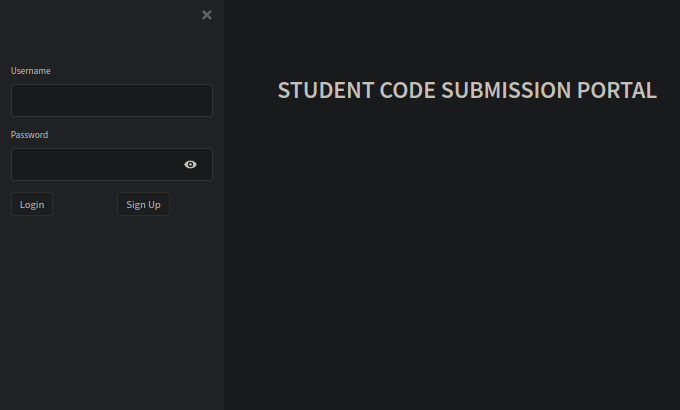
\includegraphics[scale=0.56,frame]{./figures/dep1.png}
\caption{Snippet of Student Code Submission portal before login/sign-up}
\label{fig1}
\end{figure}

\begin{figure}[H]
\centering
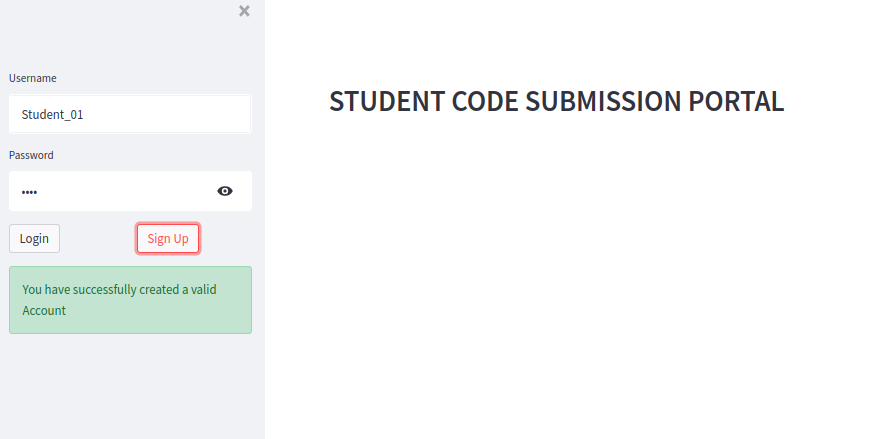
\includegraphics[scale=0.6,frame]{./figures/dep2.png}
\caption{Snippet of Student Code Submission portal after sign-up}
\label{fig1}
\end{figure}

\begin{figure}[H]
\centering
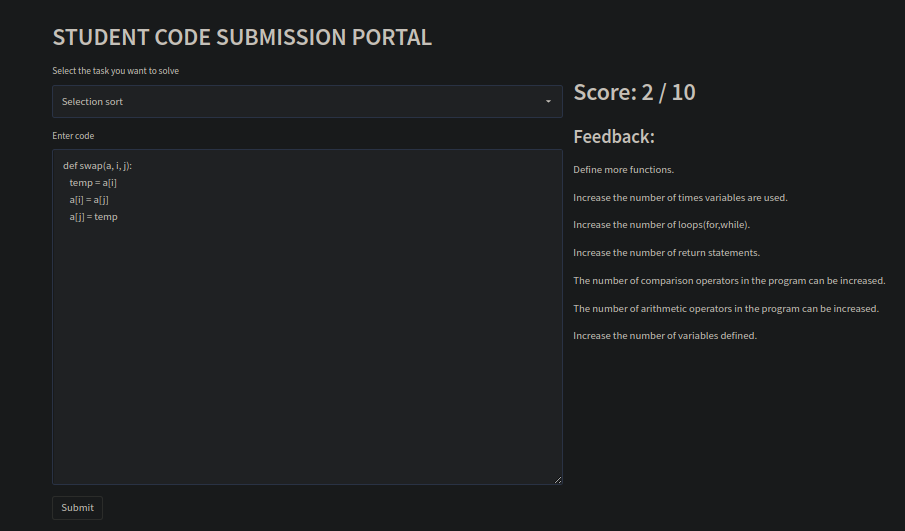
\includegraphics[scale=0.6,frame]{./figures/dep3.png}
\caption{Snippet of Student Code Submission portal after login}
\label{fig2}
\end{figure}


Figure 9.1 is the snippet of the student code submission portal before login. Since the student has not logged in yet, the tasks to be attempted are not visible.

Figures 9.2 and 9.3 is the snippet of the student code submission portal after sign-up and login. Once the student enters his username and password, the password is hashed using Secure Hash Algorithm (SHA 256) and the system checks if the user has registered already. Post successful login, the select-box and code area become visible to the student.  



\begin{figure}[H]
\centering
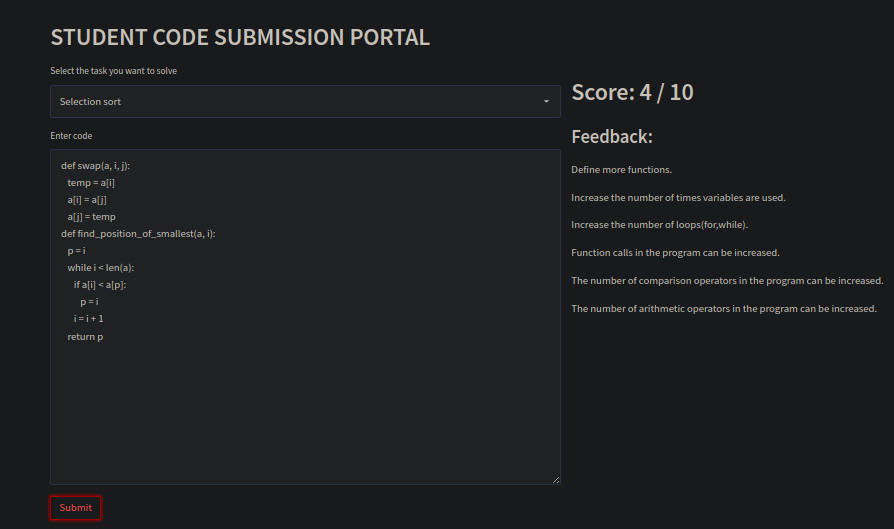
\includegraphics[scale=0.53,frame]{./figures/dep4.png}
\caption{Automatic Grading and Feedback Generation - Example 1}
\label{fig3}
\end{figure}

Figure 9.4 shows a example student submission for the selection sort task. Since the code is incomplete and only swap function is defined, the code submission is given a score of 2 out of 10. The code review feedbacks which are generated are appropriate which include suggestions like to define more functions, add more looping statements etc.

\newpage

\begin{figure}[H]
\centering
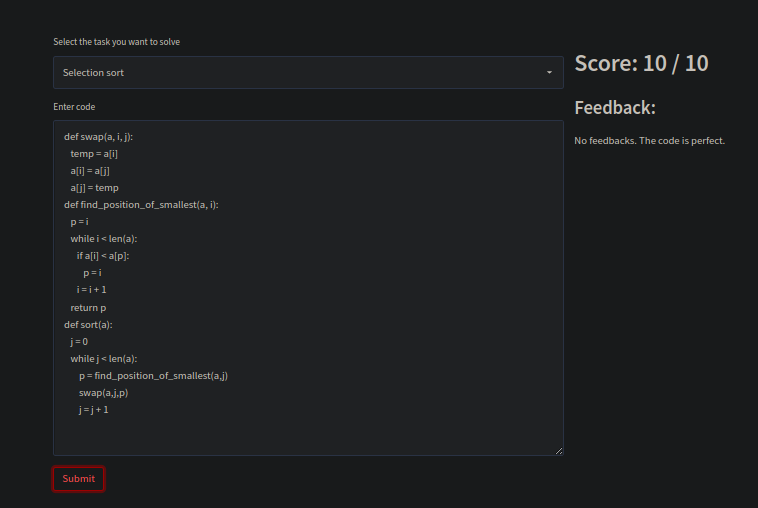
\includegraphics[scale=0.51,frame]{./figures/dep5.png}
\caption{Automatic Grading and Feedback Generation - Example 2}
\label{fig4}
\end{figure}

Figure 9.5 shows another example student submission for the election sort task. In this case, the program is incomplete again - with only two functions defined for swapping and finding the position of the smallest element in the list from a given index. Since the main sort function is missing which would have had function calls to the two defined functions and a looping statement, the code submission gets a grade of 4 out of 10 and the necessary code review feedbacks.

Figure 9.6 is another example student submission for selection sort task. In this case, the model grades the program a perfect 10/10 with no code review feedbacks. The code submission is perfect with three functions defined to perform swapping, finding the position of the smallest element from a given index and finally the sort function. The sort function includes two function calls to the previously defined functions. Thus, the model considers the particular code submission as a perfect code sample. 

\newpage

\begin{figure}[H]
\centering
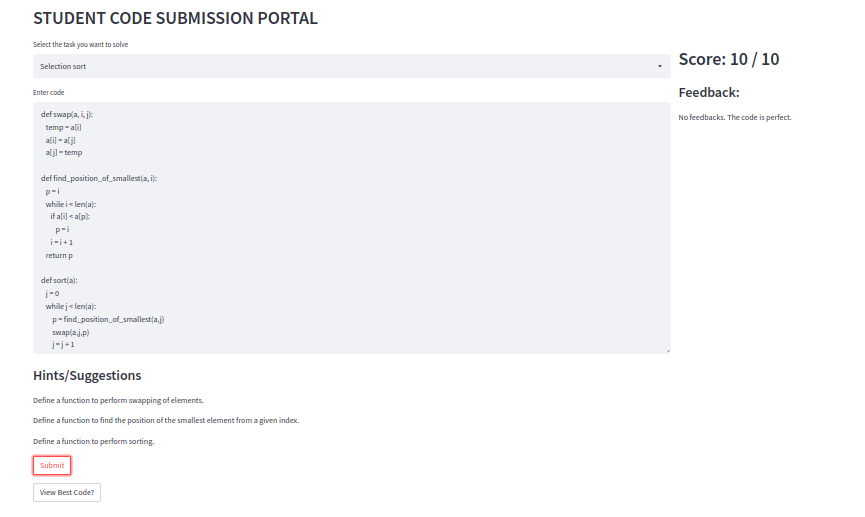
\includegraphics[scale=0.6,frame]{./figures/dep6.png}
\caption{Automatic Grading and Feedback Generation - Example 3}
\label{fig5}
\end{figure}

There is also a another feature which could prove helpful to students. As every assignments have a deadline, students can be given access to view the best  code solution after the deadline. 'View Best Code?' option gives a chance for the students to have a look into the best submission. This is shown in figure 9.7.


\begin{figure}[H]
\centering
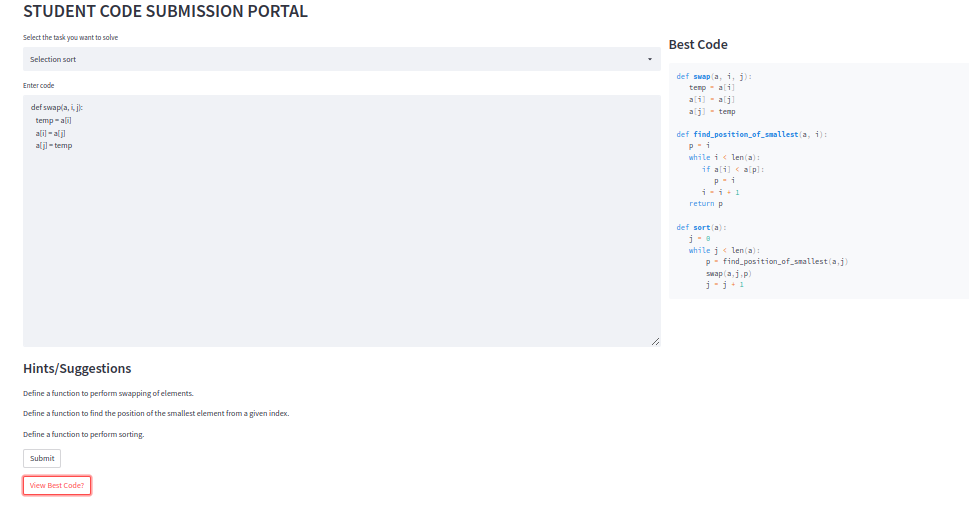
\includegraphics[scale=0.54,frame]{./figures/dep7.png}
\caption{Viewing best code submission}
\label{fig5}
\end{figure}



